\documentclass{article}

\usepackage{graphicx}
\usepackage{tikz}
\usepackage{tikzsymbols}
\usetikzlibrary{calc,patterns,shapes.geometric}
\pagestyle{empty}
\usepackage[margin=0pt]{geometry}
\geometry{papersize={14in,12in}}

\def\centerarc[#1](#2)(#3:#4:#5){\draw[#1] ($(#2)+({#5*cos(#3)},{#5*sin(#3)})$) arc (#3:#4:#5);}

\begin{document}
	\begin{figure}
		\centering
		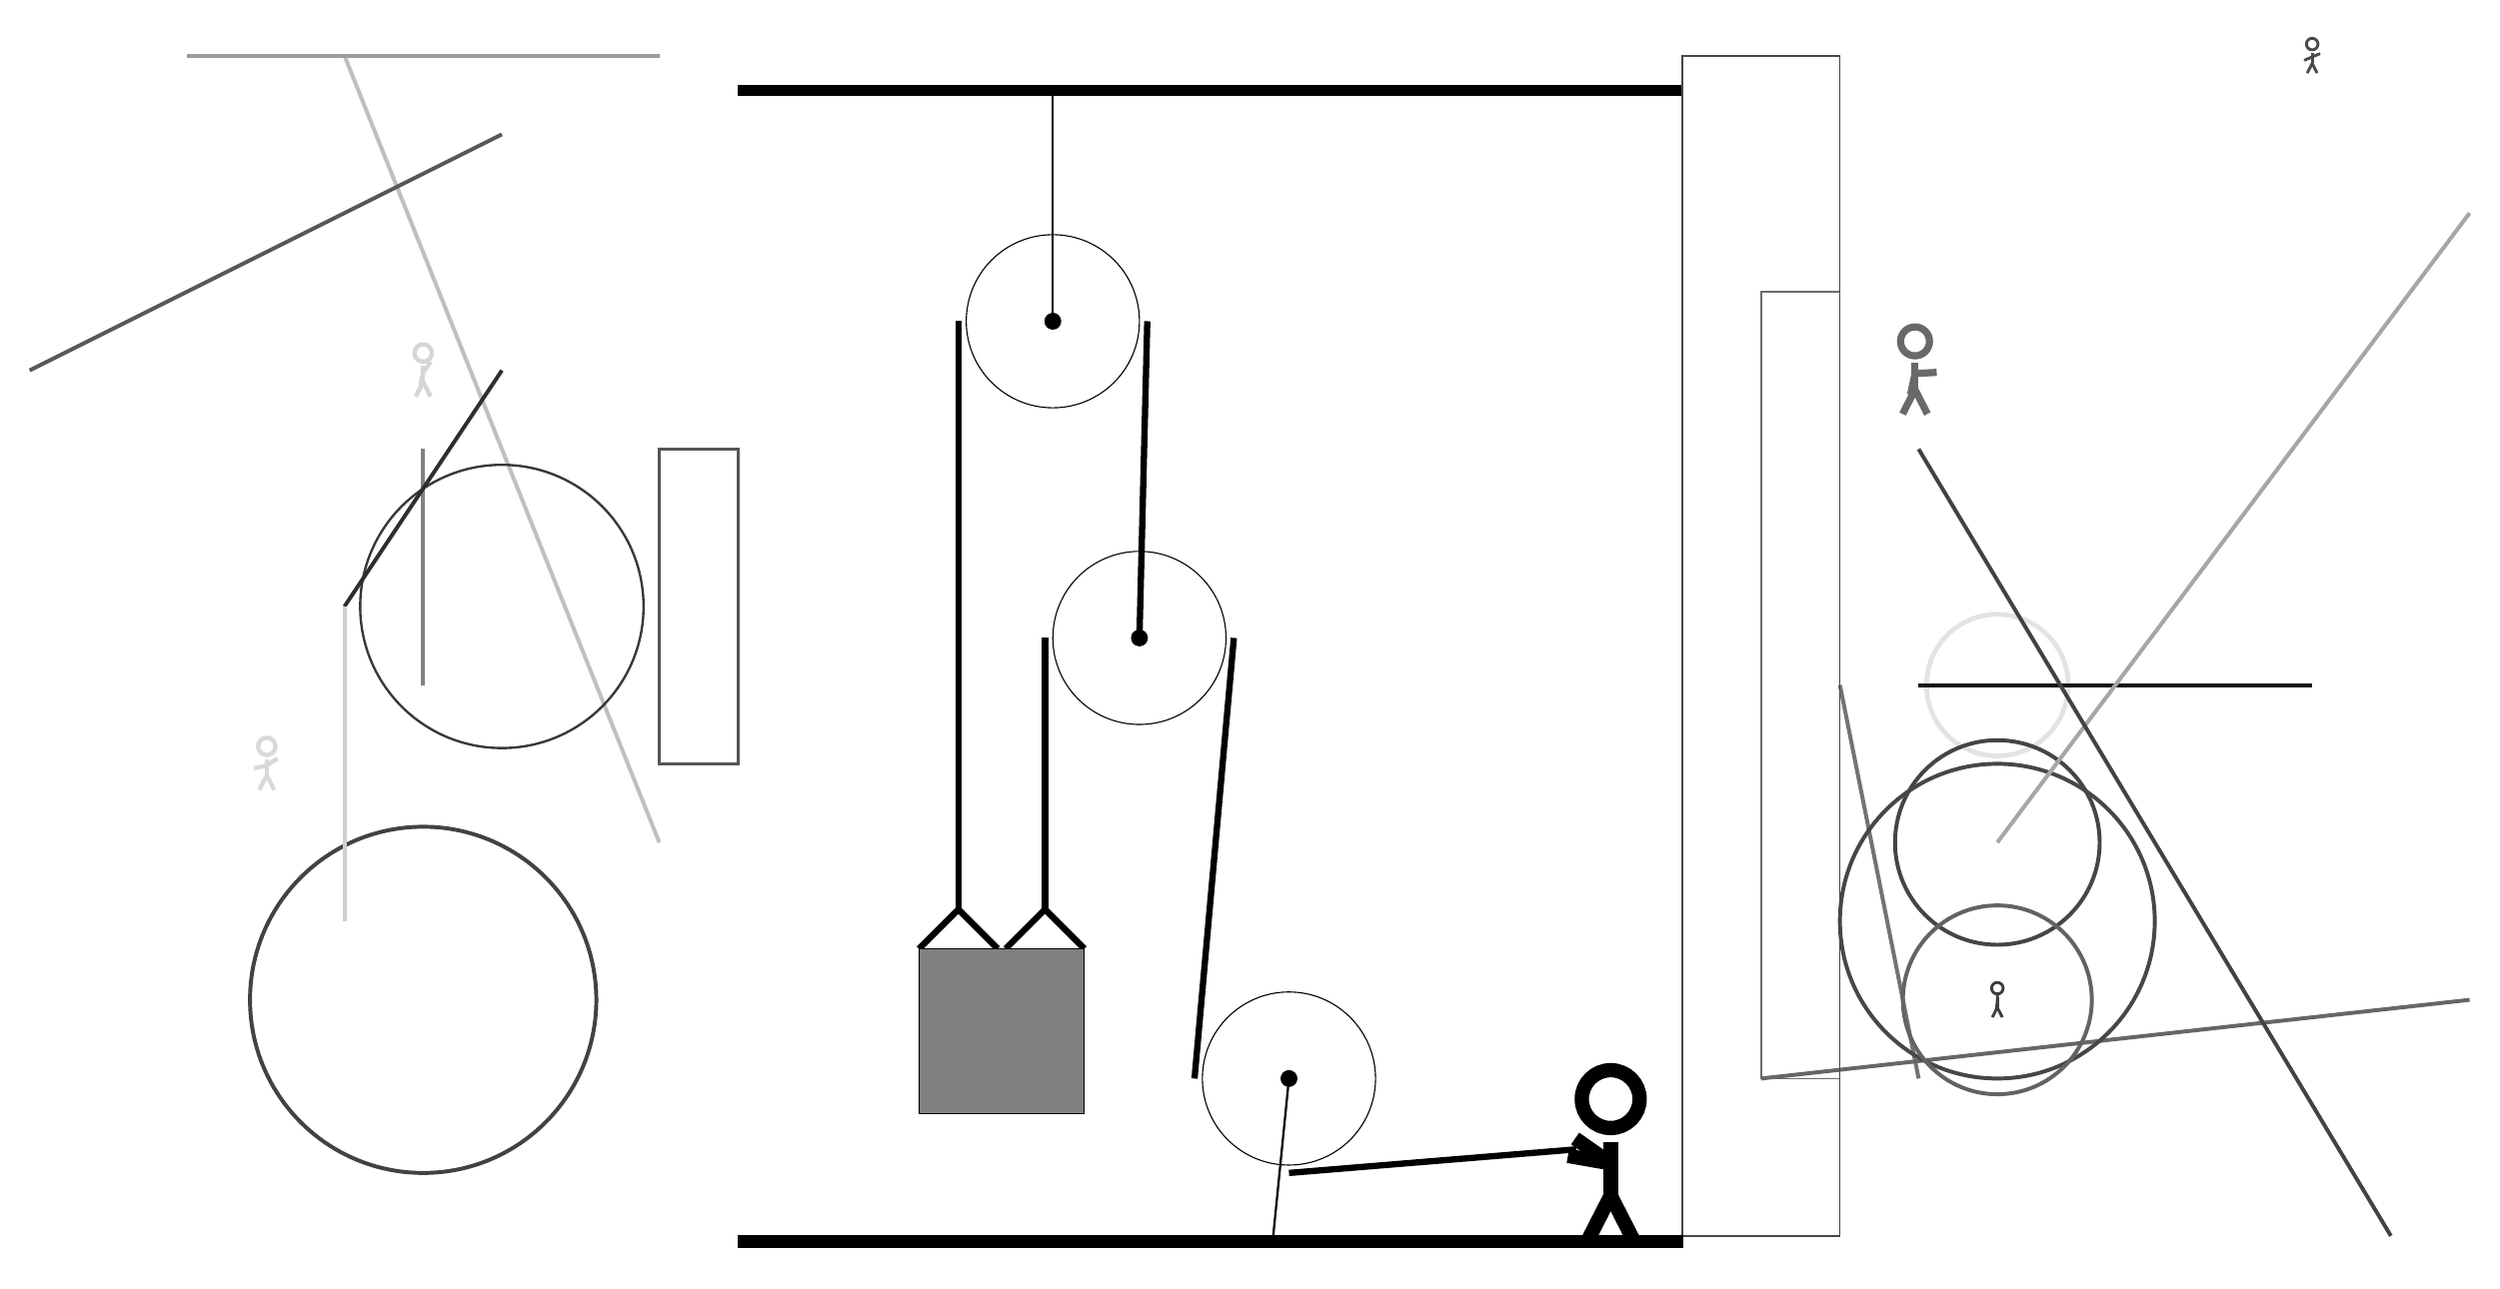
\begin{tikzpicture}
			%%%%% START %%%%%
			
			\draw[fill=black] (-2, 11.5) rectangle (10, 11.625);
			
			\draw (2, 8.625) circle (1.1);
			\draw[fill=black] (2, 8.625) circle (0.1);
			\draw[thick] (2, 8.625) -- (2, 11.5);
			
			\draw (3.1, 4.6) circle (1.1);
			\draw[fill=black] (3.1, 4.6) circle (0.1);
			
			\draw (5, -1) circle (1.1);
			\draw[fill=black] (5, -1) circle (0.1);
			\draw[thick] (5, -1) -- (4.8, -3);
			
			\draw[line width = 0.8mm]  (0.3, 0.65) -- (0.8, 1.15) -- (1.3, 0.65);
			\draw[line width = 0.8mm]  (1.4, 0.65) -- (1.9, 1.15) -- (2.4, 0.65);
			\draw[fill=black!50] (0.3, 0.65) rectangle (2.4, -1.45);
			
			\draw[line width = 0.8mm] (0.8, 8.625) -- (0.8, 1.15);
			\centerarc[line width = 0.8mm](2, 8.625)(0:180:1.2000000000000002);
			\draw[line width = 0.8mm] (3.2, 8.625) -- (3.1, 4.6);
			\draw[line width = 0.8mm] (1.9, 4.6) -- (1.9, 1.15);
			\centerarc[line width = 0.8mm](3.1, 4.6)(0:180:1.2000000000000002);
			\draw[line width = 0.8mm] (4.3, 4.6) -- (3.8, -1);
			\centerarc[line width = 0.8mm](5, -1)(180:270:1.2000000000000002);
			\draw[line width = 0.8mm] (5, -2.2) -- (8.65, -1.9);
			
			\node at (9, -2) {\Strichmaxerl[10][-35][170]};
			
			\draw[line width=0.5mm, color=black!25](-7, 12) -- (-3, 2);
			
			\draw[line width=0.5mm, color=black!55](12, 4) -- (13, -1);
			\node[line width=0.2mm, color=black!71] at (18, 12) {\Strichmaxerl[2][23][23]};
			\draw[line width=0.5mm, color=black!39](-3, 12) -- (-9, 12);
			\draw[line width=0.5mm, color=black!60](11, -1) -- (20, 0);
			\draw [line width=0.6mm, color=black!11](14, 4) circle (0.9);
			\draw [line width=0.3mm, color=black!78](-5, 5) circle (1.8);
			
			\node[line width=0.6mm, color=black!59] at (13, 8) {\Strichmaxerl[5][78][3]};
			\draw [line width=0.5mm, color=black!73](14, 2) circle (1.3);
			\draw[line width=0.5mm, color=black!65](-5, 11) -- (-11, 8);
			\draw[line width=0.5mm, color=black!90](13, 4) -- (18, 4);
			\draw[line width=0.2mm, color=black!58] (12, 9) rectangle (11, -1);
			\draw [line width=0.5mm, color=black!74](-6, 0) circle (2.2);
			\draw[line width=0.5mm, color=black!49](-6, 4) -- (-6, 7);
			\draw[line width=0.2mm, color=black!72] (10, 12) rectangle (12, -3);
			\node[line width=0.4mm, color=black!15] at (-8, 3) {\Strichmaxerl[3][11][34]};
			
			\node[line width=0.7mm, color=black!16] at (-6, 8) {\Strichmaxerl[3][78][54]};
			\draw[line width=0.4mm, color=black!67] (-3, 3) rectangle (-2, 7);
			\draw [line width=0.5mm, color=black!72](14, 1) circle (2.0);
			\draw[line width=0.5mm, color=black!82](-7, 5) -- (-5, 8);
			\node[line width=0.5mm, color=black!76] at (14, 0) {\Strichmaxerl[2][83][89]};
			
			\draw[line width=0.5mm, color=black!35](14, 2) -- (20, 10);
			\draw[line width=0.5mm, color=black!74](13, 7) -- (19, -3);
			\draw [line width=0.5mm, color=black!61](14, 0) circle (1.2);
			\draw[line width=0.5mm, color=black!19](-7, 1) -- (-7, 5);
			
			\draw[fill=black] (-2, -3) rectangle (10, -3.15);
			
			%%%%% END %%%%%
		\end{tikzpicture}
	\end{figure}	
\end{document}